\NeedsTeXFormat{LaTeX2e}
\ProcessOptions
\documentclass[a4paper]{report}

\newcommand{\nothing}{}

\RequirePackage{graphicx}
\usepackage[utf8]{inputenc}
\usepackage[T1]{fontenc}
\usepackage{textcomp}
\usepackage{mathptmx}
\usepackage[scaled=0.85]{helvet}
\usepackage{hyperref}
\usepackage{array}
\usepackage{ngerman}
\usepackage{glossaries}
\usepackage{color}
\usepackage{listings} \lstset{backgroundcolor=\color{lightgray}} \lstset{language=Java}
\usepackage{wrapfig}
\usepackage{url}
\usepackage{float}
\usepackage{natbib}
\usepackage{booktabs}
\usepackage{tabularx}
\definecolor{lightgray}{rgb}{.9,.9,.9}
\usepackage{pdfpages}

% Sylings for Tables
%%%%%%%%%%%%%%%%%%%%
\newcommand*\heading[1]{\bfseries{#1}}
\newcommand*\beforeheading{\toprule}
\newcommand*\afterheading{\midrule}
\newcommand*\normalline{}
\newcommand*\lastline{\bottomrule}


\makeindex

% do this here, so you can \gls{...} to it
%add new glossaryentries here...

\newglossaryentry{sqlite}{
	name=SQLite,
	description={SQLite ist eine Datenbankengine, welche ohne Konfiguration auskommt. Es handelt sich dabei um eine Datenbank in einer Datei},
	first={SQLite}
}
\makeglossaries


\begin{document}

\begin{titlepage}
\title{Advanced Patterns and Frameworks}
\author{Manuel Alabor}
\date{FS 2013}
\maketitle
\end{titlepage}

\tableofcontents
\newpage

% The main content
%%%%%%%%%%%%%%%%%%
\chapter{Access Control Models}
\section{Authorization}

Das Authorization Pattern beschreibt auf einfache Art und Weise die Zugriffsberechtigungen eines Subjekts auf ein bestimmtes Objekt. Es spezifiziert zudem die Art des erlaubten Zugriffes (Lesend, schreibend etc.)

\subsection*{Kontext}
Jegliche Umgebungen in denen der Zugriff auf enthaltene Objekte kontrolliert werden muss.

\subsection*{Problem}
In einer kontrollierten Umgebung muss sichergestellt werden, dass nur berechtigte Subjekte auf entsprechende Objekte zugreifen können. Es stellt sich also die Herausforderung, diese Information losgelöst von den eigentlichen Objekte abzulegen. Dabei soll aber eine gewisse Flexibilität bei der Definition von Berechtigungen, Objekten und Subjekten erhalten bleiben.

Des weiteren sollen diese Informationen so einfach wie möglich im Nachhinein änderbar sein.

\subsection*{Lösung}
Strukturell fällt die Lösung zum Authorization Pattern relativ simpel aus:

\begin{figure}[H]
	\begin{center}
	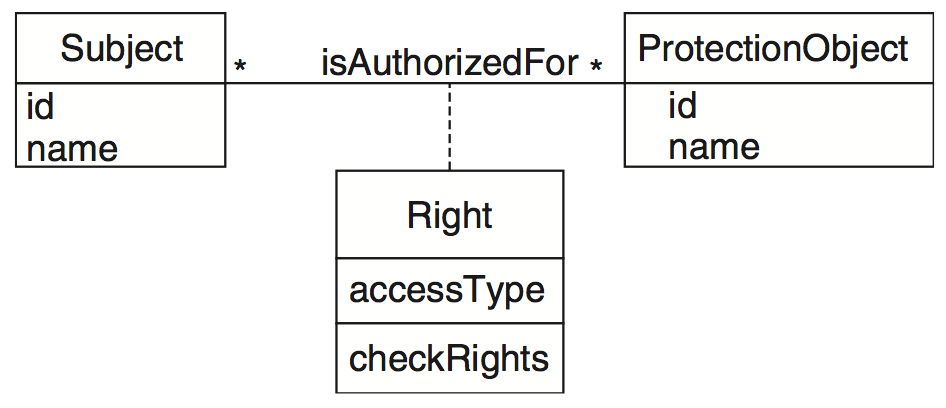
\includegraphics[width=0.75\textwidth]{chapter/01/authorization.png}
	\end{center}
	\caption{Authorization Struktur}
\end{figure}

\begin{itemize}
	\item Subject beschreibt jegliche Aspekte des zu berechtigenden Subjekts
	\item Das ProtectionObject ist das zu schützende Objekte
	\item Right enthält alle Informationen, wie Subject auf ProtectioObject zugriefen darf/kann
\end{itemize}

\subsection*{Erweiterungen}
Die vorgestellte Struktur kann um komplexere Aspekte erweitert werden. So kann bspw. mittels einem ''Copy''-Flag eine Stellvertretung eines Subjektes durch ein anderes ermöglicht werden.
Weiter ist die Verwendung eines Prädikats denkbar, welches eine Regel mit zusätzlicher ''Intelligenz'' austatten kann (-> ''Darf nur zugreifen wenn Zeit innerhalb Arbeitszeit'')

Diese Anpassungen können direkt auf dem Rights-Objekt modelliert werden.

\subsection*{Vor- \& Nachteile}
\begin{itemize}
	\item Durch seine Offen- und Allgemeinheit kann dieses Pattern auf jegliche Umgebung appliziert werden (Filesysteme, Organistaitonsstrukturen, Zugangskontrollen etc.)
	\item In der beschriebenen Form sind administrative Aufgaben (Änderung der Zugriffsrechte) nicht gesondert definiert. Für bessere Sicherheit ist dies jedoch von Vorteil
	\item Für viele Subjekte/Objekte müssen entsprechend viele Berechtigungsregeln erfasst und auch verwaltet werden
	\item Viele Regeln machen die Verwaltung für einen Administrator zu einer heiklen Aufgabe (Verkettung von Berechtigungen etc.)
\end{itemize}

\subsection*{Beispielanwendungen}
\begin{itemize}
	\item Dateisysteme
	\item Firewalls greifen teilweise auf dieses Pattern zurück, um Regeln für den analysierten Traffic zu modellieren
\end{itemize}
\section{Role Based Access Control}

Diese Pattern basiert stark auf dem Authorization Pattern und versucht dessen Nachteile durch einen zusätzlichen Abstraktionslayer auszugleichen.
Das ''Role Based Access Control'' Pattern definiert Berechtigungen nicht direkt auf Stufe der Subjekte, sondern versucht diese in Gruppen (Aufgabenbereiche, Kaderposition, Arbeitsort etc.) einzuteilen und anschliessend auf dieser Ebene quasi übergeordnet zu berechtigen.

\subsection*{Kontext}
Eine Umgebung mit vielen Objekten und Subjekten. Deren Berechtigungen ändern häufig. Zudem ist damit zu rechnen dass eben so oft neue Subjekte und Objekte hinzukommen oder wieder wegfallen.

\subsection*{Problem}
Die Rechteverwaltung in dem beschriebenen Kontext generiert einen hohen administrativen Aufwand. Um die Anzahl individueller Berechtigungen zu minimieren soll versucht werden, alle Subjekte in Gruppen einzuteilen. Die Einteilung basiert darauf, dass Subjekte mit ähnlichen Aufgaben zumeist auch ähnliche oder identische Berechtigungen benötigen.
Trotzdem sollen die Berechtigungen weiterhin präzise abgebildet werden können (''Need to know'').

\subsection*{Lösung}
Organisationen bieten normalerweise bereits mehr oder weniger wohldefinierte Gruppenstrukturen (Abteilungen, Aufgabenbereiche).
Ein gutes Sicherheitskonzept sollte bestrebt sein, dass jedes Subjekt genau auf die Objekte Zugriff hat, mit welchen es täglich arbeitet (wiederum ''Need to know'').

\begin{figure}[H]
	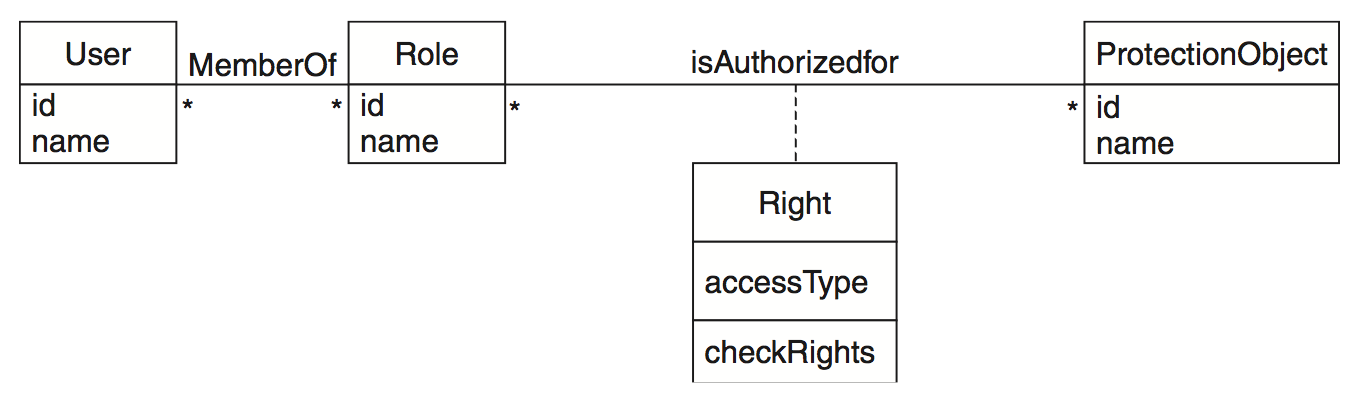
\includegraphics[width=\textwidth]{chapter/01/rolebasedaccesscontrol.png}
	\caption{Basic Role Based Access Control}
\end{figure}

Im Vergleich zum Authorization Pattern kommt lediglich ein neues Element hinzu: Die Role fasst mehrere User (Subjekte) zu einer Menge zusammen und berechtigt sie über Right für ein spezifisches ProtectionObject.


\subsection*{Erweiterungen}
\begin{figure}[H]
	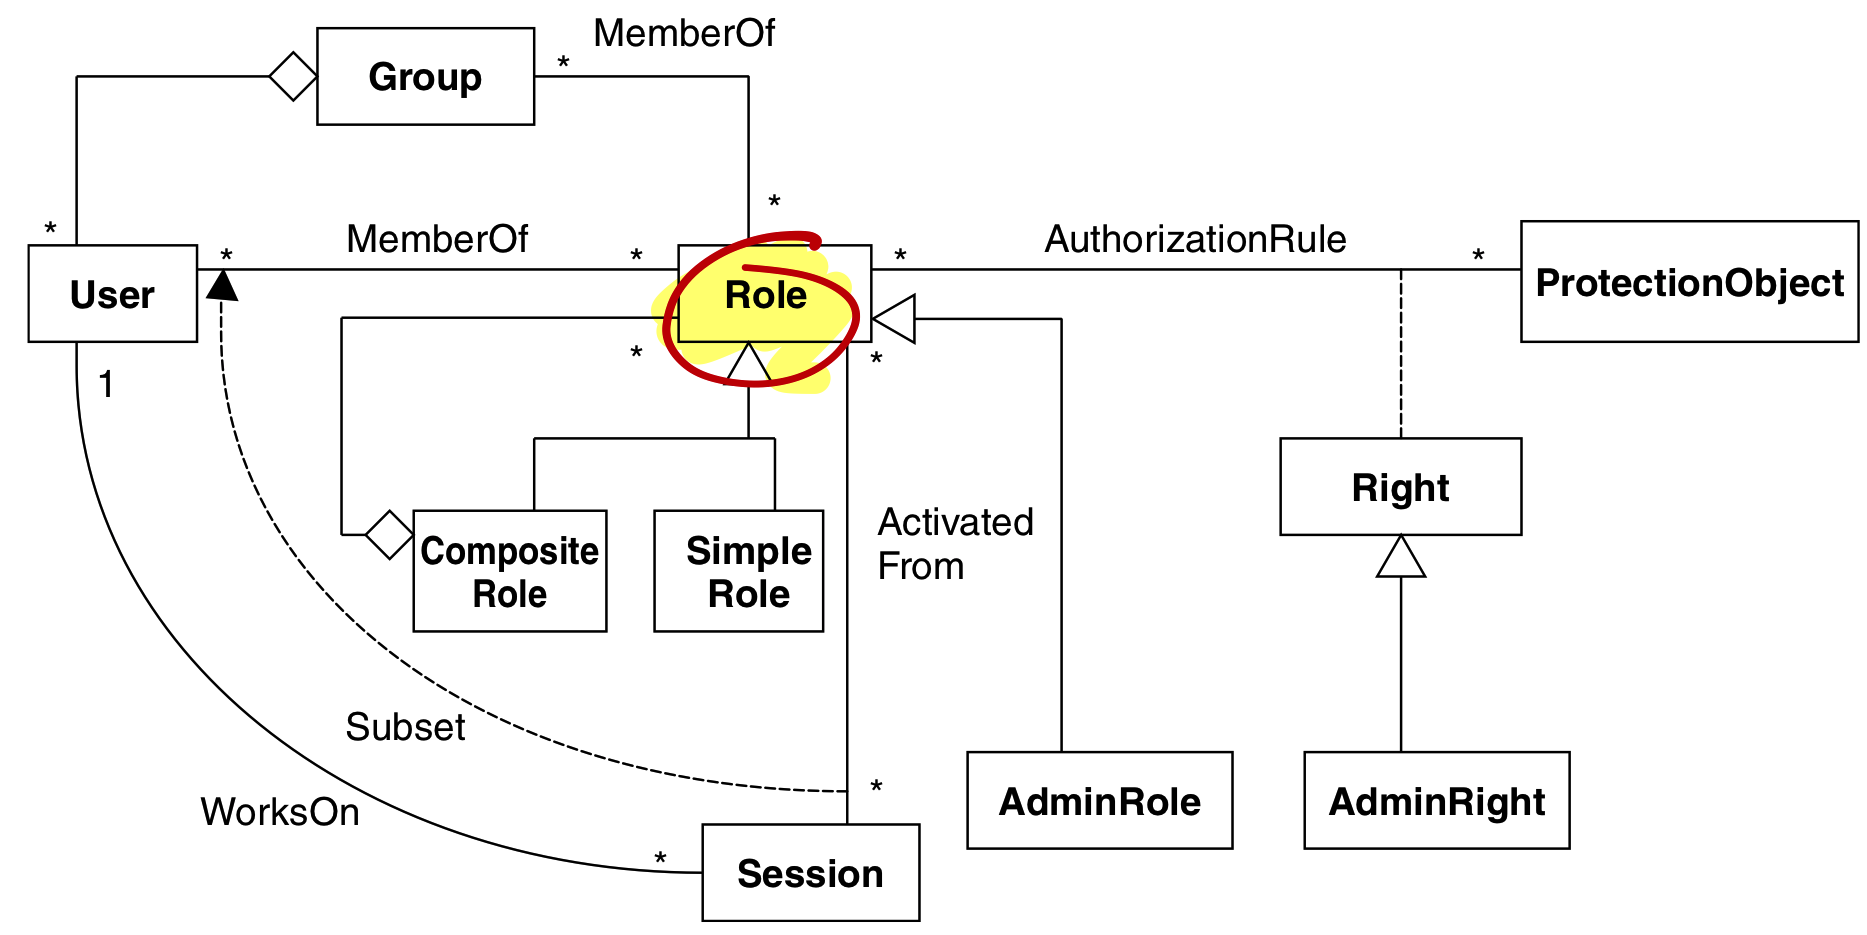
\includegraphics[width=\textwidth]{chapter/01/rolebasedaccesscontroladvanced.png}
	\caption{RBAC mit Composite, Admins \& Abstract Session}
\end{figure}

\subsubsection*{Composite Pattern}
Statt einer simplen Assoziation zwischen User und Role könnte auch mit dem Composite-Pattern gearbeitet werden, um diese Abhängigkeit zu modellieren.

\subsubsection*{Administration}
Wie ebenfalls bereits im Authorization-Pattern erwähnt kann auch dieses Modell zielgerichtet um Administrations-Elemente erweitert werden.
Auf diese Weise kann zusätzliche Klarheit im System geschaffen werden, wer genau für was zuständig ist.

\subsubsection*{Abstract Session}
Um die Möglichkeiten auf die Spitze zu treiben, sei hier auch das Abstract Session Pattern erwähnt: Die Abhängigkeit einer Session kann so direkt ins Security Modell ''miteinmodelliert'' werden.

\subsection*{Vor- \& Nachteile}
\begin{itemize}
	\item Die Zusammenfassung zu Gruppen ermöglicht eine vereinfachte Administration der gesamthaft vorhandenen Berechtigungen
	\item Veränderungen in der realen Organistaionstruktur (Neuzugänge, Abgänge, Jobwechsel etc.) können einfacher auf das Sicherheitskonzept abgebildet werden
	\item Ein Subjekt kann durch mehrere Sessions verschiedene Funktionen auf einmal wahrnehmen
	\item Theoretisch können Gruppen wiederum in Gruppen zusammengefasst werden (Yay, even more complexity...)
	\item Konzeptionelle Komplexität nimmt durch die neuen Elemente wiederum zu!
\end{itemize}

\subsection*{Beispielanwendungen}
\begin{itemize}
	\item Windows 2000 Rights Management (Group Policies)
	\item 
\end{itemize}

\chapter{Workshop Notizen}
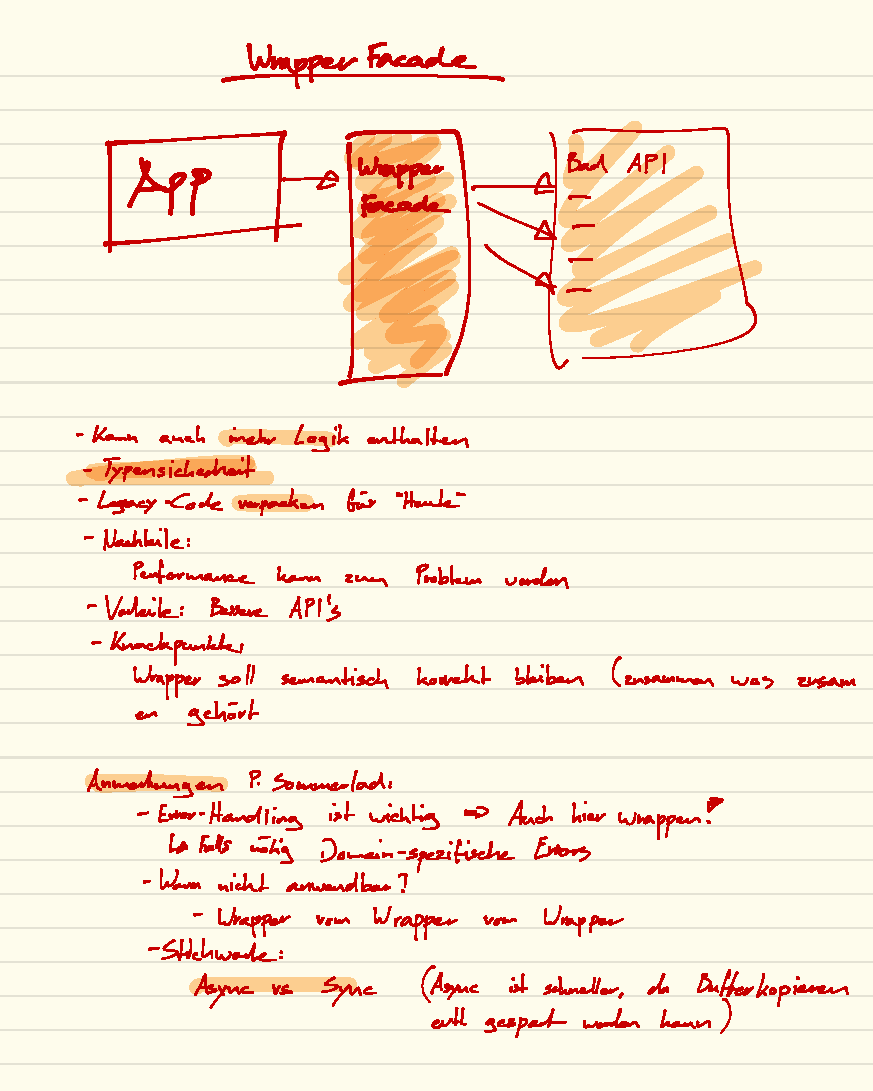
\includepdf[pages=-,pagecommand=\thispagestyle{plain},scale=0.75]{chapter/99/Workshops.pdf}

% List of figures & glossary
%%%%%%%%%%%%%%%%%%%%%%%%%%%%
\listoffigures
\printglossary[style=altlist,title=Glossar]

% Bibliography
%%%%%%%%%%%%%%
\bibliographystyle {alpha}
\bibliography{index/bibliography}

\end{document}